\documentclass[12pt]{report}

% Import packages
\usepackage{listings}  % For adding C code
\usepackage{xcolor}    % For custom colors
\usepackage{graphicx}  % For including images
\usepackage{amsmath}   % For advanced math formatting
\usepackage{hyperref}  % For creating hyperlinks
\usepackage{geometry}  % To set page margins
\usepackage{subfig}
\geometry{a4paper, margin=1in}

\usepackage{pgfplots}
\pgfplotsset{compat=1.18} % Adjust version if needed

\lstdefinestyle{cstyle}{
    language=C,
    basicstyle=\ttfamily\footnotesize, % Font style
    keywordstyle=\color{purple}\bfseries, % Keywords in blue
    stringstyle=\color{orange}, % Strings in red
    commentstyle=\color{olive}, % Comments in gray
    numbers=none, % No line numbers
    tabsize=4, % Tab space width
    showspaces=false,
    showstringspaces=false,
    frame=single, % Adds a single-line box around the code
    framerule=0.8pt, % Thickness of the frame
    framesep=5pt, % Space between frame and code
}

\begin{document}

\title{\textbf{Bitonic Sort with MPI}}
\author{Ioannis Michalainas, Savvas Tzanetis}
\maketitle

\tableofcontents  % Generates the table of contents

\chapter{Abstract}
This report is part of an assignment for the \textbf{Parallel and Distributed Systems} class of the
Aristotle University's Electrical and Computer Engineering department. This project implements a
distributed sorting algorithm using a \textbf{Bitonic Sort} implementation. 

The primary objective is to sort a dataset of N = $2^{q+p}$ processes in ascending \newline order
utilizing the \textbf{Message Passing Interface (MPI)} for inter-process communication. The
implementation leverages parallel processing to achieve efficient sorting, making it suitable for
large-scale data sets. Key components include vector operations, extremum calculations, and min-max
comparisons, all orchestrated to perform the bitonic sort in a distributed environment.

\chapter{Bitonic Algorithm}
    \section{Serial}
        \subsection{Explanation}
        In order to be able to fully understand how the bitonic algorithm works, we first need to explain what is a \textbf{bitonic sequence}. A \textbf{bitonic sequence}, is a sequence of numbers that first increases and then decreases, or vise versa. For example the sequence:
        \[
            \{3, 8, 12, 18, 24, 27, 31, 35, 34, 29, 25, 20, 15, 10, 6, 2\}
        \]
        Is a bitonic sequence, where the numbers increase up to the \textbf{elbow} number
        \textbf{35}, and later decrease.        
        
        Now that we have successfully shown what a bitonic sequence is, we can begin describing a 
        serial implementation of the \textbf{Bitonic sort} algorithm. The Bitonic Sort algorithm is a 
        comparison-based sorting algorithm that organizes the elements of a random sequence into a
        bitonic one. More specifically:

        The first step in the bitonic sorting algorithm is to divide the unsorted array into smaller 
        subsequences and arrange them into bitonic sequences. After forming these bitonic sequences,
        the algorithm sorts them by repeatedly comparing and swapping elements in pairs so that one 
        half of the sequence becomes entirely smaller than the other half. After this step, the sorted
        halves are merged recursively and the same process starts again, comparing pairs of numbers
        from subsequences and swapping the correct elements. The algorithm operates recursively,
        breaking down the sorting into smaller bitonic sorts and merges. The steps are applied
        repeatedly with different step sizes until the entire array is sorted.

        The time complexity of this algorithm is \(\boldsymbol{O(n \log^2(n))}\), which while it is
        higher than most sorting algorithms like \textbf{Merge Sort} or \textbf{Quick Sort}, It is
        well-suited for parallelization techniques, like the one we will be discovering later.

        \newpage
        \subsection{Example}
        Using a random sequence we can illustrate an example:
        \[80, 37, 44, 23, 66, 63, 34, 17, 45, 54, 43, 33, 46, 92, 7, 50 \]
        The first step would be splitting the above sequence of
        numbers into \textbf{2 subsequences}. After that, we will be left with:
        \[
            S_1 = \{80, 37, 44, 23, 66, 63, 34, 17\}, \quad S_2 = \{45, 54, 43, 33, 46, 92, 7, 50\}
        \]
        And then recursively, split the two subsequences again to:
        \[
            \begin{array}{cc}
                S_1 = \{80, 37, 44, 23\} & S_2 = \{66, 63, 34, 17\} \\
                S_3 = \{45, 54, 43, 33\} & S_4 = \{46, 92, 7, 50\}
            \end{array}
        \]
        And sort them, alternating between ascending and descending order for each of our sequences:
        \[
            \begin{array}{cc}
                S_1 = \{23, 37, 44, 80\} & S_2 = \{66, 63, 34, 17\} \\
                S_3 = \{33, 43, 45, 54\} & S_4 = \{92, 50, 46, 7\}
            \end{array}
        \]
        Pairing $S_1$ with $S_2$ and $S_3$ with $S_4$, we then merge the pairs into two sequences, the first in ascending order and the second in descending:
        \[
            S_1 = \{17, 23, 34, 37, 44, 63, 66, 80\}, \quad S_2 = \{92, 54, 50, 46, 45, 43, 33, 7\}
        \]
        And lastly, merging the two halves again in ascending order:
        \[
            S_1 = \{7, 17, 23, 33, 34, 37, 43, 44, 45, 46, 50, 54, 63, 66, 80, 92\}
        \]

        The merging process involves comparing each element in the pair of subsequences. For an ascending order, the first subsequence retains the smaller elements from each comparison, while the second subsequence retains the larger elements. For a descending order, the process is reversed: the first subsequence retains the larger elements, and the second subsequence retains the smaller elements. After comparing all elements in the pairs, the subsequences are merged back together.
        
        
    \newpage
    \section{Distributed}
    As previously mentioned, this algorithm, when implemented in a serial manner, has a time complexity of \(\boldsymbol{O(n\log^2(n))}\), which is larger than most sorting algorithms. Despite this fact, this algorithm is useful as it is well-suited for distributed implementations like the one we will be discussing. This means, that for a parallel implementation, we can achieve a time complexity of \(\boldsymbol{O(\log^2(n))}\), which is significantly faster than our serial implementation. We will be achieving this goal, by utilizing the \textbf{Message Passing Interface (MPI)} for inter-process communication, allowing us to distribute the load across multiple machines.
    
        \subsection{Generating Random Sequences}
        The sequence we are using to test our results are being generated via the use of the \textbf{rand()} function, which is part of the \textbf{C standard library}. More specifically the max number we allow to be added to a sequence is \textbf{999} for simplicity, as well as it being recommended for this assignment.
        \begin{lstlisting}[style=cstyle]
void randomVec(Vector* vec, int max) {
    srand(time(NULL));
    for (int i=0; i<vec->size; i++) {
        vec->arr[i] = rand()%max;
    }
}
        \end{lstlisting}
        Here, Vector is a struct we implemented with two variables, \textbf{arr} for storing the data and \textbf{size} for storing the size of the array \textbf{arr}.
        
        \subsection{MPI Communication}
        This algorithm is implemented in a parallel manner, by distributing the computing load to different machines using the \textbf{MPI}
        protocol. MPI, also allows to simulate multiple machines, by creating different process to a single computer running the same code. Each process is given an \textbf{ID} called \textbf{"rank"}, and is generally working independently from other processes, except for times where synchronization is needed. In the code below we can see how such processes are created using \textbf{MPI}:
        \begin{lstlisting}[style=cstyle]
// run a copy of main for each rank
MPI_Init(&argc, &argv);
int rank, size;
MPI_Comm_rank(MPI_COMM_WORLD, &rank);
MPI_Comm_size(MPI_COMM_WORLD, &size);
        \end{lstlisting}\newpage
        Generating different processes isn't enough though, these processes, or \textbf{ranks}, should also be able to communicate with each other, in order to exchange data and synchronize. Luckily, the MPI library already provides us with these necessary functions: 
        \begin{lstlisting}[style=cstyle]
// Rank 0 Scatters data to all other ranks
MPI_Scatter(data->arr, local->size, MPI_INT, local->arr,
            local->size, MPI_INT, 0, MPI_COMM_WORLD);

// Other ranks accept data but don't send anything themselves
MPI_Scatter(NULL, local->size, MPI_INT, local->arr, 
            local->size, MPI_INT, 0, MPI_COMM_WORLD);
        \end{lstlisting}
        In the case above, \textbf{data} holds the randomly generated array that awaits to be sorted, while \textbf{local} represents the sub-arrays of each rank that will be handling the bitonic sort locally.
        \vfill
        Lastly, since a crucial step in the Bitonic sorting process is merging subsequences, a rank should be responsible for storing this data in its \textbf{local} array, after gathering data from its neighboring rank. This is done with the use of the exchange function:
        \begin{lstlisting}[style=cstyle]
void exchange(int partner, Vector* local, Vector* remote) {

  MPI_Sendrecv(local->arr, local->size, MPI_INT, partner, 0,
               remote->arr, local->size, MPI_INT, partner, 0,
               MPI_COMM_WORLD, MPI_STATUS_IGNORE);
}
        \end{lstlisting}
        \subsection{Bitonic Implementation}
        In this sub-section, we will be discussing how this algorithm has been implemented in a distributed manner.

        First and foremost, after the random array data has been distributed across all ranks, each rank will run through an initial sorting process that will only be run once, as instructed by the assignments requirements. This sorting is done using the \textbf{qsort} function provided by the C standard library like so:
        \begin{lstlisting}[style=cstyle]
void initialSort(Vector* local, int rank) {
  if (rank & 1) {
    qsort(local->arr, local->size, sizeof(int), compDescending);
  } else { 
    qsort(local->arr, local->size, sizeof(int), compAscending);
  }
}
        \end{lstlisting}
        Where \textbf{(rank \& 1)} is a logical operation, essentially allowing us to sort the sub-arrays into descending and ascending order, alternating between the two options.

        After this process, we run two for loops, one nested to the other, where the first will be executed \textbf{p} times, as \textbf{p} is the numbers of \textbf{steps} needed to sort a full array for a sequence size \textbf{n}, where \[p = log_2(n)\].
        Inside these loops, using logical operations, we calculate the distance a rank should have with its neighboring partner, as well as what rank that partner has.
        \newpage
        \begin{lstlisting}[style=cstyle]
for (int stage=1; stage<=p; stage++) {
    for (int step=stage; step>=1; step--) {
      int distance = 1 << (step-1);
      int partner = rank ^ distance;

      exchange(partner, local, remote);
      minmax(rank, stage, distance, local, remote);
    }
    // Ascending (0) or Descending (1)
    int direction = (rank & (1 << stage)) == 0;     
    elbowmerge(local, direction);
  }
        \end{lstlisting}
        The function \textbf{minmax} is responsible for sorting each pair of numbers in the rank pairs to \textbf{min} and \textbf{max} arrays, as previously shown in the serial implementation more specifically:
        \begin{lstlisting}[style=cstyle]
void minmax(int rank, int stage, int distance, 
            Vector* local, Vector* remote) {
  int mirror = 1 << stage;
  int w = 2*mirror;
  int pos = rank % w;

  int reflection = pos<mirror ? mirror-pos - 1 : pos-mirror; 

  if (reflection & (1 << (int)log2(distance))) {
    min(local, remote);
  } else {
    max(local, remote);
  }
}
        \end{lstlisting}
        The functions \textbf{min} and \textbf{max} are simple functions used for switching the numbers of a local
        \vspace{0.5cm}
        array with the remote one if either the min or max requirements are met.
        
        Lastly, the \textbf{elbowmerge}, will run \textbf{p} times and is responsible
        for merging two halves of a bitonic sequence into a single sorted sequence, in either ascending or
        \vspace{0.5cm}
        descending order.

        In the code below, we use a \textbf{struct} called \textbf{Extremum}, which holds the point index of the
        \vspace{0.5cm}
        extremum point in a bitonic sequence as well as its polarity (if it is min or max).

        This is done by comparing every point in the array in \textbf{O(n)} time. It is also worth noting that in
        extreme cases where an array doesn't have an extremum point (i.e \textbf{4 4 2 2}, the \textbf{elbow} function
        always returns the largest number as a \textbf{max extremum} point.
        \newpage
        \begin{lstlisting}[style=cstyle]
void elbowmerge(Vector* local, int direction) {
  Extremum point = elbow(local);
  int  n   = local->size;
  int* tmp = malloc(sizeof(int)*n);

  int left  = (point.index-1 + n) % n;
  int right = (point.index+1) % n;

  if (point.polarity == -1) {  
    int i = 0;
    tmp[i++] = local->arr[point.index];  

    while (i < n) {
      if (local->arr[left] < local->arr[right]) {
        tmp[i++] = local->arr[left];
        left = (left-1 + n) % n;  // move left index circularly
      } else {
        tmp[i++] = local->arr[right];
        right = (right + 1) % n;  // move right index circularly
      }
    }
  } else if (point.polarity == 1) {  
    int i = n-1;
    tmp[i--] = local->arr[point.index];  

    while (i >= 0) {
      if (local->arr[left] > local->arr[right]) {
        tmp[i--] = local->arr[left];
        left = (left-1 + n) % n;  // move left index circularly
      } else {
        tmp[i--] = local->arr[right];
        right = (right+1) % n;  // move right index circularly
      }
    }
  }
  if (direction == 1) {
    memcpy(local->arr, tmp, sizeof(int)*n);
  } else {
    for (int j=0; j<n; j++) {
      local->arr[j] = tmp[n-1 - j];
    }
  }
  free(tmp);
}
        \end{lstlisting}

\chapter{Results}
    As previously mentioned, a serial version of this algorithm has a times complexity of \(\boldsymbol{O(n \log^2(n))}\), which
    is not ideal, as there are faster algorithms, but a parallel or distributed version, significantly lessens this to 
    \(\boldsymbol{O(\log^2(n))}\).

    We tested these algorithms with \textbf{33.554.432} (or $2^{25}$) random numbers in a sequence, ranging between the numbers 
    \textbf{1 - 999}. This is done because the bitonic sorting algorithm can successfully sort only sequences in the 
    \textbf{power of 2}. The algorithms where run inside the \textbf{Aristotle Cluster} provided by the \textbf{Aristotle University of Thessaloniki}, with \textbf{4 cores}, splitting the load among \textbf{4 processes} or \textbf{ranks.}

\begin{table}[h!]
    \centering
    \begin{tabular}{|c|c|c|c|}
        \hline
        \rule{0pt}{3ex}\textbf{Performance Table} & \textbf{Serial}                 & \textbf{Distributed}          & \textbf{Quick Sort}          \\ \hline
        \rule{0pt}{3ex}Time Complexity            & \(\boldsymbol{O(n \log^2(n))}\) & \(\boldsymbol{O(\log^2(n))}\) & \(\boldsymbol{O(n\log(n))}\) \\ \hline
        \rule{0pt}{3ex}Time(Seconds)              & \textbf{1}min \textbf{51}sec    & \textbf{6.02}sec              & \textbf{1}min \textbf{24}sec \\ \hline
    \end{tabular}
    \caption{Performance Table.}
    \label{tab:simple_table}
\end{table}

\begin{center}
    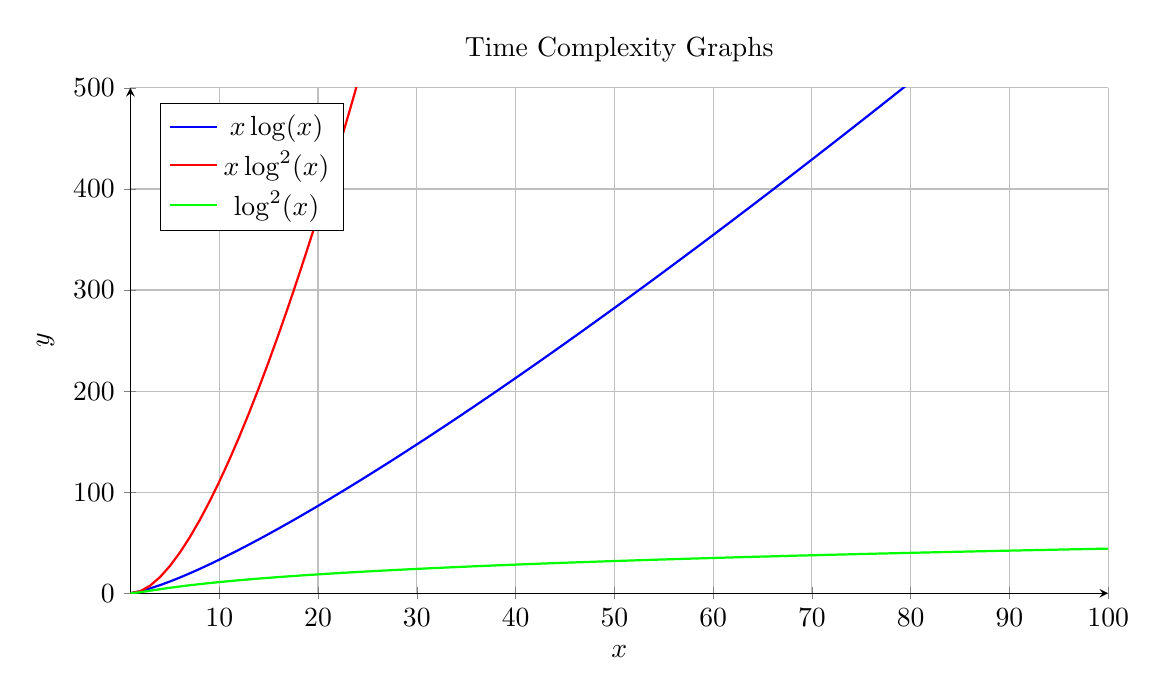
\begin{tikzpicture}
        \begin{axis}[
            width=14cm, % Set the width of the plot
            height=8cm, % Set the height of the plot
            xlabel={$x$},
            ylabel={$y$},
            xmin=1, xmax=100, % Range for x-axis
            ymin=0, ymax=500, % Adjust y-axis range for visibility
            legend pos=north west,
            grid=major,
            axis x line=bottom,
            axis y line=left,
            title={Time Complexity Graphs}
        ]
            % Plot x * log2(x)
            \addplot[blue, thick] expression[domain=1:100, samples=100]{x * ln(x)/ln(2)};
            \addlegendentry{$x \log(x)$}

            % Plot x * (log2(x))^2
            \addplot[red, thick] expression[domain=1:100, samples=100]{x * (ln(x)/ln(2))^2};
            \addlegendentry{$x \log^2(x)$}

            % Plot (log2(x))^2
            \addplot[green, thick] expression[domain=1:100, samples=100]{(ln(x)/ln(2))^2};
            \addlegendentry{$\log^2(x)$}
        \end{axis}
    \end{tikzpicture}
\end{center}
    As we can see our distributed implementation of the \textbf{Bitonic Sort} algorithm is significantly faster than a serial implementation, as well as other serial sorting algorithms like \textbf{Quick Sort}.

\chapter{Tools and Sources}
    In this project, the following tools where used:
    \begin{enumerate}
        \item The \textbf{C} programming language.
        \item The \textbf{OpenMPI} Library for implementing the distributed algorithm.
        \item \textbf{GitHub} for version control.
        \item \textbf{GitHub Copilot} as an AI assistant.
    \end{enumerate}
    While the following sources were helpful in understanding of the problem presented in the assignment.
    \begin{itemize}
        \item \url{https://en.wikipedia.org/wiki/Bitonic_sorter}
        \item Lecture notes from the \textbf{Parallel and Distributed Systems} course, written by professor \textbf{Nikolaos Pitsianis}.
    \end{itemize}

\end{document}
